% !TEX TS-program = pdflatexmk
\documentclass[12pt]{amsart}
\usepackage{multicol}
\usepackage{float}

%\usepackage[parfill]{parskip}    % Activate to begin paragraphs with an empty line rather than an indent

\usepackage[margin=1in]{geometry}


\usepackage{amsmath,amssymb,amsthm,latexsym,graphicx}
\usepackage[normalem]{ulem}
\usepackage{setspace} %used for doublespacing, etc.
\usepackage{hyperref}
\usepackage{cancel}
\usepackage[dvipsnames,usenames]{color}
\usepackage[all]{xy}
\usepackage{fancyhdr}
\pagestyle{fancy}
	\renewcommand{\headrulewidth}{0.5pt} % and the line
	\headsep=1cm
	
\DeclareGraphicsRule{.tif}{png}{.png}{`convert #1 `dirname #1`/`basename #1 .tif`.png}

%Some useful environments.
\newtheorem{theorem}{Theorem}
\newtheorem{corollary}[theorem]{Corollary}
\newtheorem{conjecture}[theorem]{Conjecture}
\newtheorem{lemma}[theorem]{Lemma}
\newtheorem{proposition}[theorem]{Proposition}
\newtheorem{definition}[theorem]{Definition}
\newtheorem{example}[theorem]{Example}
\newtheorem{axiom}{Axiom}
\theoremstyle{remark}
\newtheorem{remark}{Remark}
\newtheorem*{exercise}{Exercise}%[section]

%Some useful shortcuts for our favorite fields
\def\RR{\ensuremath{\mathbb R}} %Note, you can use these WITHOUT entering math mode
\def\NN{\ensuremath{\mathbb N}}
\def\ZZ{\ensuremath{\mathbb Z}}
\def\QQ{{\ensuremath\mathbb Q}}
\def\CC{\ensuremath{\mathbb C}}
\def\EE{{\ensuremath\mathbb E}}

%Some useful shortcuts for formatting lists
\newcommand{\bc}{\begin{center}}
\newcommand{\ec}{\end{center}}
\newcommand{\be}{\begin{enumerate}}
\newcommand{\ee}{\end{enumerate}}
\newcommand{\bi}{\begin{itemize}}
\newcommand{\ei}{\end{itemize}}

%Some useful shortcuts for formatting mathematical symbols
\newcommand{\ol}[1]{\overline{#1}}
\newcommand{\oimp}[1]{\overset{#1}{\iff}} %labeled iff symbol
\newcommand{\bv}[1]{\ensuremath{ \vec{\mathbf{#1}}} } %makes a vector.
\newcommand{\mc}[1]{\ensuremath{\mathcal{#1}}} %put something in caligraphic font
\newcommand{\mpg}[1]{\marginpar{ #1}} %to put comments in margins
\newcommand{\bsl}[1]{\texttt{\symbol{92}{\em #1}}} %for backslashes.
\newcommand{\normale}{\trianglelefteq}
\newcommand{\normal}{\triangleleft}

%Code for formatting the proofs a little nicer for submitted homework
\makeatletter
\renewenvironment{proof}[1][\proofname]{\par\doublespacing
  \pushQED{\qed}%
  \normalfont \topsep6\p@\@plus6\p@\relax
  \list{}{%
    \settowidth{\leftmargin}{\itshape\proofname:\hskip\labelsep}%
    \setlength{\labelwidth}{0pt}%
    \setlength{\itemindent}{-\leftmargin}%
  }%
  \item[\hskip\labelsep\itshape#1\@addpunct{:}]\ignorespaces
}{%
  \popQED\endlist\@endpefalse
  \singlespacing
}
\makeatother


%Commenting tools. You can ignore this stuff unless we're exchanging materials where I'm commenting in detail on how you are writing/using LaTeX.
\usepackage{soul}
\definecolor{highlight}{rgb}{1,0.6,0.6}
\sethlcolor{highlight}
\newcommand{\hlm}[1]{\colorbox{highlight}{$\displaystyle #1$}}
\newtheoremstyle{mycomment}{\topsep}{-0in}{\small \itshape \sffamily}{}{\small \itshape\sffamily}{:}{.5em}{}
\theoremstyle{mycomment}
\newtheorem*{acomment}{\color{BrickRed}{Comment}}
\newcommand{\com}[1]{{\color{OliveGreen}\begin{acomment}{#1} %#2 \color{black} 
\end{acomment}\noindent}}
%\newcommand{\com}[1]{{\color{BrickRed}{\\ Comment:}\color{OliveGreen}{#1} \\}}
\newcommand{\red}[1]{{\color{BrickRed} #1}}
\newcommand{\blue}[1]{{\color{MidnightBlue}#1}}
\newcommand{\green}[1]{{\color{OliveGreen}#1}}
\newcommand{\mwrong}[2]{\red{\cancel{#1}}\green{#2}}
\newcommand{\wrong}[2]{\red{\sout{#1}}\green{#2}}
\definecolor{OliveGreen}{rgb}{.3,.5,.2}
\definecolor{MidnightBlue}{rgb}{.3,.4,.6}
\newcommand{\pts}[1]{\hfill\blue{{#1}/5}}

\chead{MATH 631F}
\pagestyle{fancy}
%Modify these items:
\rhead{\emph{Stefano Fochesatto}}
\lhead{\emph{HW \#5 --- \today}}

\DeclareMathOperator{\lcm}{lcm}
\begin{document}

\thispagestyle{fancy}
\author{Coordinator: Coordinator's Name}



%3.3 1, 3, 7.
%3.4 4, 5, 6.
%3.5 3, 6, 10.
%Extra credit: 3.5.4.





\section*{\textbf{Section 3.3}}


\begin{exercise}[\textbf{3.3.1}] Let $F$ be a finite field of order $q$ and let $n \in \ZZ^+$. Prove that $|GL_n(F): SL_n(F)| = q - 1$
  \begin{proof} Suppose $F$ is a finite field of order $q$. Let $n \in \ZZ^+$ and consider $GL_n(F)$ and $SL_n(F)$. Recall from exercise $3.1.35$ of Homework 3 where we showed that $GL_n(F)\trianglelefteq SL_n(F)$ showing that the map $f: GL_n(G) \to F^*$ defined by $f(A) = det(A)$ was a homomorphism (albeit a dubious argument stating $det(AB) = det(A)det(B)$ by some property of determinants). We continued by applying the First Isomorphism theorem to state that $GL_n(F)/S_n(F) \cong F^*$. Since $F^*$ has order $q - 1$ this demonstrates that $|GL_n(F): SL_n(F)| = q - 1$. 
  \end{proof}
\end{exercise}
\vspace{.15in}



\begin{exercise}[\textbf{3.3.3} - Stefano Fochesatto] Prove that if $H$ is a normal subgroup of $G$ of prime index $p$ then for all $K \leq G$ either $\textbf{(i)}$ $K \leq H$ or $\textbf{(ii)}$ $G = HK$ and $|K: K \cap H| = p$.\\
  \begin{proof}
      Suppose $H$ is a normal subgroup of $G$ of prime index $p$ and $K \leq G$. Note that since $H \trianglelefteq G$ we know that $N_G(H) = G$ and further that $K \leq N_G(H)$. By the Second Isomorphism Theorem it then follows that $KH/H \cong K/K \cap H$, and $H \leq KH \leq G$. We demonstrated in class that if $H \leq KH \leq G$ then $|G:H| = |G:KH||KH:H|$. Since $KH/H \cong K \cap H$ we know that 
      $|KH:H| = |K:K\cap H|$. Therefore by substitution we get, 
      \begin{equation*}
        |G:KH||KH:H| = |G:KH||K:K\cap H| = |G:H| = p.
      \end{equation*}
      $\textbf{(i)}$ Suppose that $|G:KH| = p$ and $|K:K\cap H| = 1$. Therefore for every $k \in K$, $k K \cap H = 1  K \cap H$. So $k \in K \cap H$ and therefore $k \in H$. Thus $K \leq H$.\\

      \noindent $\textbf{(ii)}$ Suppose that $|G:KH| = 1$ and $|K:K\cap H| = p$. Therefore for every $g \in G$, $gKH = 1KH$. Therefore $g \in KH$ and $G \leq KH$. Since $KH \leq G$ from the Second Isomorphism Theorem, it follows that $G = KH$. Recall that Proposition 14 gives us that $HK = KH$ if either is a subgroup of $G$. Hence $G = HK$. 
    \end{proof}
\end{exercise}
\vspace{.15in}



\begin{exercise}[\textbf{3.3.7}] Let $M$ and $N$ be normal subgroups of $G$ such that $G = MN$. Prove that 
  $G/(M \cap N) \cong (G/M) \times (G/N)$[Draw the Lattice].
  \begin{proof} Suppose $M$ and $N$ are normal subgroups of $G$ such that $G = MN$. Consider the mapping $\varphi: G \to  (G/M) \times (G/N)$ defined by $\varphi(g) = (gM, gN)$. Note that $\varphi(ab) = (abM, abN) = (aM, aN)(bM, bN) = \varphi(a) \varphi(b)$ (the operation $aMbM = abM$ is well defined by Proposition 5,  Section 3.1). Thus $\varphi$ is a homomorphism and clearly any element $g \in M \cap N$ will map to $(M, N)$, the identity. Hence $ker(\varphi) = M \cap N$. Since $G = MN$ every $g \in G$ can be written as a product $g = mn$ for some pair $m\in M$ and $n \in N$. Thus for any pair of cosets $(g_1M, g_2N)$ we know there exists some $m_1, m_2\in M$ and $n_1, n_2 \in N$ such that $(g_1M, g_2N) = (m_1n_1M, m_2n_2N)$. Since $M$ is a normal subgroup we can simplify,
    \begin{equation*}
      (g_1M, g_2N) = (m_1n_1M, m_2n_2N) = (Mm_1n_1,  m_2n_2N) = (Mn_1,  m_2N) = (n_1M,  m_2N) = \varphi(n_1m_2). 
    \end{equation*}
    Thus $\varphi$ is a surjective homomorphism. Applying the First Isomorphism Theorem we get that $G/(M \cap N) \cong (G/M) \times (G/N)$.
    \begin{figure}[H] %\usepackage{float}
      \begin{center}
        \caption{Lattice Diagram for $G$. Dashed lines denote normal relationship.}
        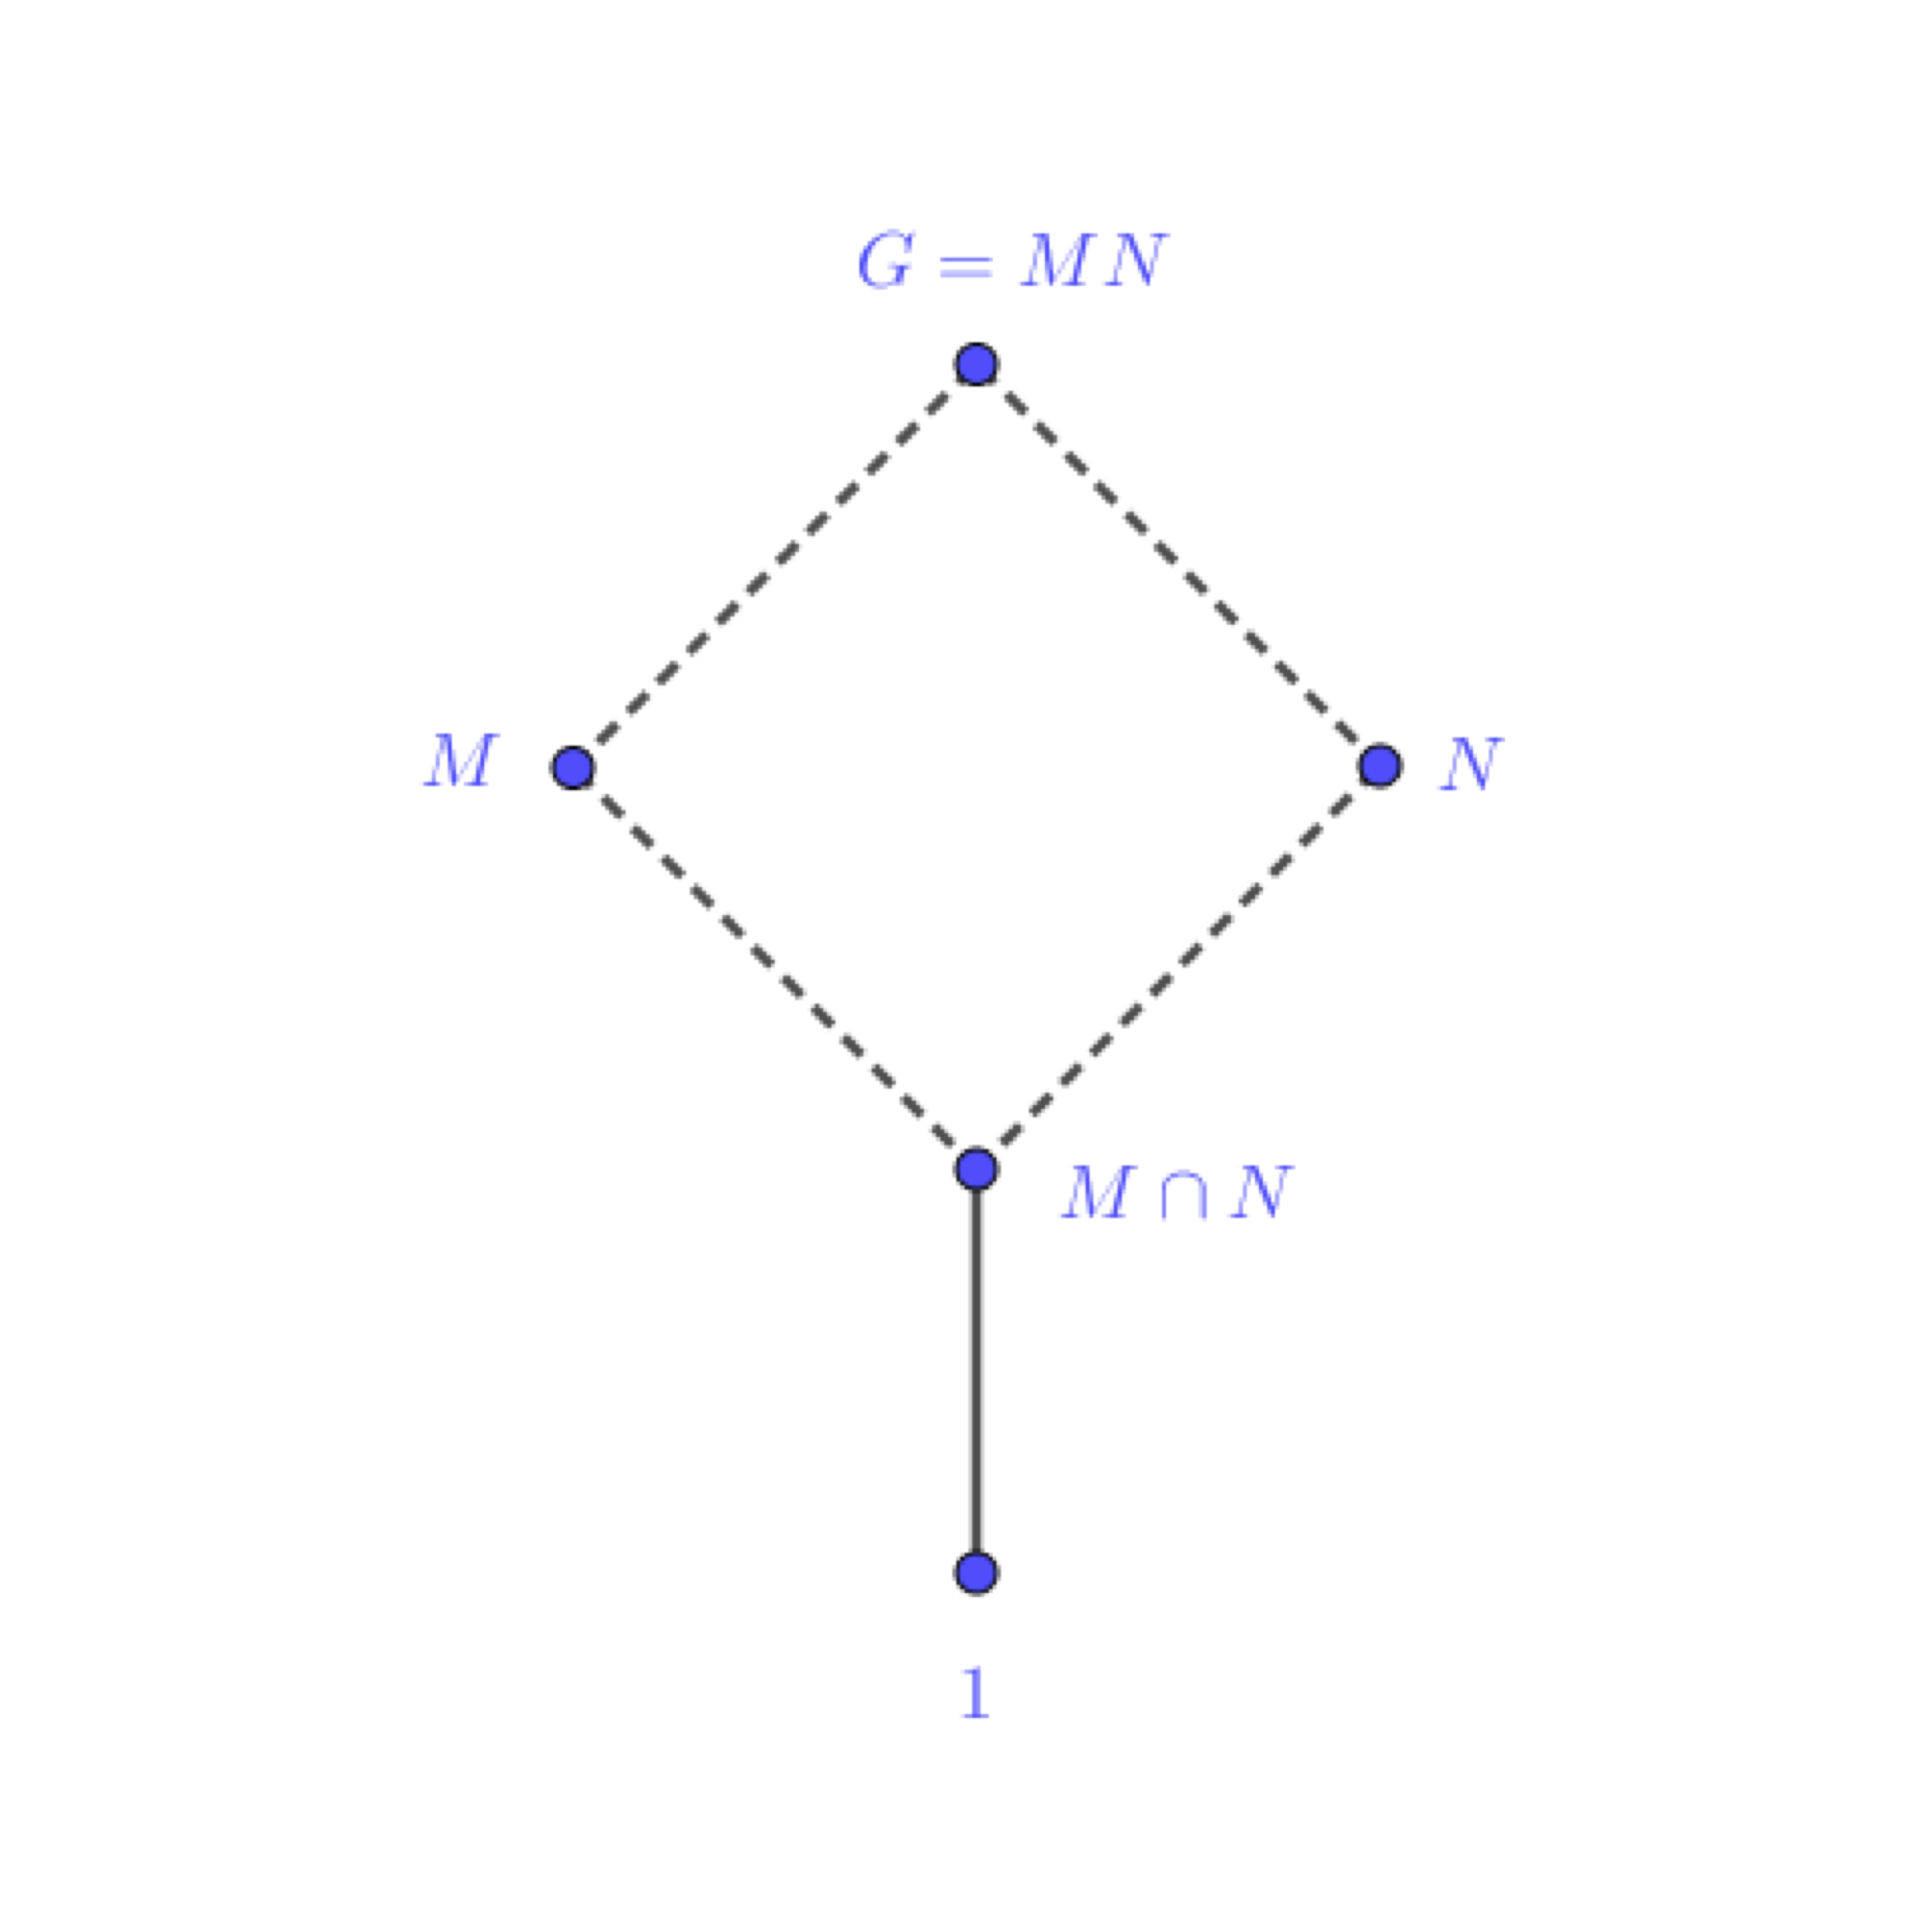
\includegraphics[width=.5\textwidth]{Lattice1.png}
      \end{center}
    \end{figure} 
  \end{proof}
\end{exercise}
\vspace{.15in}

\section*{\textbf{Section 3.4}}



\begin{exercise}[\textbf{3.4.4}] Use Cauchy's Theorem and induction to show that a finite abelian group has a subgroup of order $n$ for each positive divisor $n$ of its order.\\
  \begin{proof} Let $G$ be a finite abelian group. Clearly if $|G| = 1$ then the statement holds, there exists a subgroup, with order of each divisor of $1$. 
    Also note that for prime orders of $G$ the statement holds, namely subgroups $1$ and $G$, since $p$ has no other divisors.\\

    We continue via strong induction on $|G| = n$. Suppose that for all $k$ from $1 \leq k < n$ there exists subgroups $H_i \leq G_k$ where $|H_i|$ is 
    a divisor of $|G_k| = k$.\\
    Let $d$ be a divisor of $G_n$. If $d$ is prime then by Cauchy's Theorem it follows that there exists some element $x \in G_n$ such that $|x| = d$,
    therefore $|\langle x\rangle| = d$ and we have our subgroup. If $d$ is not prime then there exists some prime $p$ such that $d = jp$ where $j \in \ZZ$. 
    By Cauchy's Theorem there exists some $x \in G_n$ such that $|\langle x\rangle| = p$. Now consider $G_n/\langle x\rangle$ and sincd all our groups are finite recall that by Lagrange's Theorem, 
    $|G_n/\langle x\rangle| = |G_n|/|\langle x\rangle| = n/p$. Note that $|G_n/\langle x\rangle| < |G_n| = n$ and has order with divisor $j$. Thus by the inductive hypothesis, there exists some subgroup
    $H \leq G_n/\langle x\rangle$ such that $|H| = j$. Since $G_n$ is abelian $\langle x\rangle$ is normal in $G_n$, therefore by the Lattice Isomorphism Theorem, $H$ is of the form $H/\langle x\rangle$ for some $H \leq G_n$. Note that by Lagrange's Theorem $|H/\langle x\rangle| = |H|/|\langle x\rangle| = j$, and therefore $|H| = jp = d$.
  \end{proof}
\end{exercise}
\vspace{.15in}



\begin{exercise}[\textbf{3.4.5}] Prove that subgroups and quotient groups of a solvable group are solvable. 
  \begin{proof} Let $G$ be a solvable group and $H \leq G$. Since $G$ is solvable we know that there exists 
    a chain of subgroups, 
    \begin{equation*}
      1 = G_0 \trianglelefteq G_1 \trianglelefteq G_2 \trianglelefteq \dots \trianglelefteq G_s = G
    \end{equation*}
    such that $G_{i + 1}/G_i$ is abelian for $0 \leq i \leq s - 1$. Consider the set of subgroups of $H$, $H_i = (H \cap G_i)$
    with $0 \leq i \leq s$. For $H$ to be solvable we must show that $H_i \trianglelefteq H_{i + 1}$ and $H_{i + 1}/H_i$ is abelian.
    Let $h_1 \in H_i$ and $h_2 \in H_{i+1}$. Note that since $G_i \trianglelefteq G_{i + 1}$ we know that $h_2h_1h_2^{-1} \in G_i$, and clearly 
    $h_2h_1h_2^{-1} \in H$. Thus $h_2h_1h_2^{-1} \in H_i$ and we conclude that $H_i \trianglelefteq H_{i + 1}$.\\
    Next consider the quotient group $H_{i + 1}/H_i = (H \cap G_{i + 1})/(H \cap G_{i})$. Note that since $H_i \trianglelefteq H_{i + 1} \trianglelefteq H$ we know that $H_i = H \cap G_{i} = H_{i + 1} \cap G_{i}$. By substitution we get $H_{i + 1}/H_i = H_{i + 1}/H_{i + 1} \cap G_{i}$. Clearly $H_{i + 1} \leq N_g(G_i) = G$ and thus by the Second Isomorphism Theorem we know that $H_{i + 1}/H_{i + 1} \cap G_{i} \cong H_{i + 1}G_i/G_i$, $G_i \trianglelefteq H_{i + 1}G_i$, and $H_{i + 1}G_i \leq G$.
    Note that $H_{i + 1}G_i/G_i = (G_{i + 1}\cap H)G_i/G_i \leq G_{i + 1}/G_i$ since $(G_{i + 1}\cap H)G_i \leq G_{i + 1}$. Since $H_{i + 1}G_i/G_i$ is a subgroup of an abelian group it must also be abelian, and therefore $H_{i + 1}/H_i$ is abelian. Thus $H$ is solvable\\

    Let $N \trianglelefteq G$ consider $\bar{G} = G/N$. By The Fourth Isomorphism Theorem (We need $N \trianglelefteq G$ for this) there exists a bijection from 
    the set of subgroups of $G$ which contain $N$ and the set of subgroups of $G/N$. Since $G$ is solvable there must exist a chain of normal subgroups of $\bar{G}$ where $\bar{G_i} = G_i/N$ such that $N \leq G_i$, 
    \begin{equation*}
      1 = \bar{G_0} \trianglelefteq \bar{G_1} \trianglelefteq \bar{G_2} \trianglelefteq \dots \trianglelefteq \bar{G_s} = \bar{G}. 
    \end{equation*}
    Now we must demonstrate that $\bar{G_{i + 1}}/\bar{G_{i}}$. Note that $N, G_i \trianglelefteq G_{i + 1}$ (This comes from $N \trianglelefteq G$ and $N \subseteq G_i$) therefore by the Third Isomorphism Theorem we 
    conclude that $\bar{G_{i + 1}}/\bar{G_{i}} = (G_{i + 1}/N)(G_{i}/N) \cong G_{i + 1}/G_{i}$. Since $G$ is solvable $G_{i + 1}/G_{i}$ is abelian and therefore 
    $\bar{G_{i + 1}}/\bar{G_{i}}$ is also abelian. Thus $G/N$ is solvable.
  \end{proof}
\end{exercise}
\vspace{.15in}





\begin{exercise}[\textbf{3.4.6}] Prove $(1)$ of the $Jordan-H\ddot{o}lder$ $Theorem$ by induction on $|G|$. If $G$ is a finite group with $|G| \neq 1$ then $G$ has a composition series. 
  \begin{proof} Let $G$ be a finite group with $|G| \neq 1$. We will proceed by induction on $|G| = n$. Consider 
    the base case, $|G| = 2$. Clearly the group $G$ is composed of two elements $G = \{1, g\}$ with $g^{-1}g = 1$. 
    Consider the composition series, $1 \leq G$. 

    Now suppose for all $|G| = k$ such that $2 \leq k < n$ there exists a composition series. Let $|G| = n$. Consider a proper normal subgroup $H$. By the Induction Hypothesis $H$ has a composition series, 
    \begin{equation*}
      1 \leq H_0 \leq H_1 \leq \dots \leq H_m = H
    \end{equation*}
    Note that all $H_i \leq G$. Now consider $\bar{G} = G/H$. Since $H$ is a proper normal subgroup we know that $|\bar{G}|<n$. Thus by the Induction Hypothesis there exists a composition series, 
    \begin{equation*}
      H \leq \bar{G}_1 \leq \bar{G}_2 \leq \dots \leq \bar{G}_i = G.
    \end{equation*}
    By the Fourth Isomorphism Theorem there exists a bijection $\varphi$ from the set of subgroups of $G$ which contain $H$ and the set of subgroups of $\bar{G}$. So let $\varphi^{-1}(\bar{G}_i) = G_i$ and note it also follows from the Fourth Isomorphism Theorem since $\bar{G}_{i} \trianglelefteq \bar{G}_{i + 1}$ we know that $G_i \trianglelefteq G_{i + 1}$. Finally note that by the Third Isomorphism Theorem we know that $\bar{G}_{i + 1}/\bar{G}_{i} \cong G_{i + 1}/G_{i}$. Thus the composition factors for $G_i$ are simple, giving us the following composition series, 
    \begin{equation*}
      H \leq G_1 \leq G_2 \leq \dots \leq G_i = G.
    \end{equation*}
    Finally by substitution we get the following composition series for $G$
    \begin{equation*}
      1 \leq H_0 \leq H_1 \leq \dots \leq H_m = H \leq G_1 \leq G_2 \leq \dots \leq G_i = G.
    \end{equation*}
  \end{proof}
\end{exercise}
\vspace{.15in}



\section*{\textbf{Section 3.5}}



\begin{exercise}[\textbf{3.5.3}] Prove that $S_n$ is generated by $\{(i (i+1))| 1 \leq i \leq n - 1\}$ 
  \begin{proof} Let $G$ be the group generated by $\langle\{(i (i+1))| 1 \leq i \leq n - 1\}\rangle$. We will proceed by induction on $|S_n| = n$. Consider the base case, let $n = 2$. Clearly $G$ contains all elements from $S_2$ i.e. $(1 2)$ and $(1 2)^2$. Suppose that for all $2 \leq k < n$, $S_k = G_k = \langle\{(i (i+1))| 1 \leq i \leq k - 1\}\rangle$. Let $a \in S_n$ and note that $a$ can be written as a product of transpositions. Let all transpositions that comprise $a$ be of the form $(a_1 a_2)$. If $a_1, a_2 \in [n - 1]$ then clearly by the induction hypothesis $(a_1 a_2) \in G_{n - 1} \leq G_n$. Similarly if $a_1 = n - 1$ and $a_2 = n$ then by definition $(a_1, a_2) \in G_n$. Consider the case where $a_1 \in [n - 1]$ and $a_2 = n$. With conjugates we see that $(a_1 n) = ((n - 1) n)(a_1 (n - 1))((n - 1) n) \in G_n$. Since every transposition of $S_n$ is in $G_n$, it follows that $a \in G_n$. 
  Thus $S_n$ is generated by $G_n$. 
    \end{proof}
\end{exercise}
\vspace{.15in}


\begin{exercise}[\textbf{3.5.6}] Show that $\langle (1 3), (1 2 3 4) \rangle$ is a proper subgroup of $S_4$. What is the isomorphism type of this subgroup?
  \begin{proof} Let $G = \langle (1 3), (1 2 3 4) \rangle$. Note that $(1 3)^2 = (1 2 3 4)^4 = 1$, and $(1 2 3 4)(1 3) = (1 3)(1 2 3 4)$. Note that these generators function identically to $r, s \in D_{2(4)}$. Consider the map $\varphi: D_{2(4)} \to G$ defined by $\varphi(r) = (1 2 3 4)$ and $\varphi(s) = (1 3)$. This map is clearly an isomorphism, hence $|G| = |D_{2(4)}| = 8$. With $|G| = 8$, $G$ must be a proper subgroup of $S_4$ since $|S_4| = 24$. 
    \end{proof}
\end{exercise}
\vspace{.15in}




\begin{exercise}[\textbf{3.5.10}] Find a composition series for $A_4$. Deduce that $A_4$ is solvable. 
  \begin{proof}[Solution] Consider the subset of $A_4$, $G = \{1, (12)(34), (13)(24), (14)(23)\}$. We will demonstrate that $G \trianglelefteq A_4$. First note that for any pair $(a b)(c d), (a d)(b c) \in G$ the product is the third $(a b)(c d)(a d)(b c) = (ac)(db)$. Since $(ac)(db) = (ca)(bd)$ we get that $G$ is also abelian. Also note that each element is it's own inverse. Therefore $G \leq A_4$. Note that for any $a \in A_4$ we can treat it as a bijective map from $a:[4] \to [4]$. Clearly any $aGa^{-1}$ will result in permutation of the form $(a b)(c d)$ so $G\trianglelefteq A_4$.
    Since $G$ is abelian we know all subgroups of $G$ must be normal. Thus we get the following composition series (we can double check with the lattice diagram at the end of Section 3.5), 
    \begin{equation*}
      1 \leq \langle(12)(34)\rangle \leq G \leq A_4. 
    \end{equation*} 
    Note that $|\langle(12)(34)\rangle/1| = 2$, $|G/\langle(12)(34)\rangle| = 2$, and $|A_4/G| = |A_4|/|G| = 3$. Note that with the orders of every composition factor being even, they are all cyclic and therefore abelian. Thus $A_4$ is solvable. 
    \end{proof}
\end{exercise}
\vspace{.15in}





\end{document} 



